\section{The Science of Technical Exploitation}

In the early 1990s there were no DF tools as we know them
today. Instead practitioners had to repurpose tools that had been
developed for other purposes. For example, backup software was
used for collection and preservation, while data recovery tools were used
for examining subject media. Although these approaches worked, they lacked control,
repeatability, and a known error rates---that is, examiners had no way
of knowing the accuracy of their results. 

In 1993 the US Supreme Court held in the case of Daubert v. Merrell
Pharmaceutical 
that any scientific testimony presented in court must be based on a theory
that is testable; that has been scrutinized and found favorable by the
scientific community; that has a known or potential error rate; and
that is generally accepted\cite{daubert}. This case didn't directly
kick off the demand for DF tools, but it did give DF practitioners
grounds for arguing that validated tools were needed not just as a matter
of good science and procedure, but as a matter of law. 

Since then there has been a steady development of techniques and the
incorporation of those techniques in a variety of tools. This section
presents several techniques for what has come to be called
\emph{technical exploitation}. The first two techniques---hashing and
file extraction---now dominate all DF processing. The next three
techniques---reconstruction of compressed data, memory parsing, and
fraud detection in multimedia---represent the next generation of DF
research that is leveraging new algorithms and signal processing
approaches to help address challenges facing DF practitioners today.

\subsection{Files Recovery and File carving}

Many forensic investigations start with the examiner looking for
files belonging to the computer's previous user. But what is a file?

On modern digital systems, a \emph{file} is a sequence of
\emph{bytes}. Files therefore
have \emph{contents} and a \emph{length}, but they do not necessarily have other
information that computer users typically associate with files, such
as a \emph{file name} or a \emph{modification date}. These attributes
are called \emph{metadata} (literally ``data about data'')
and are stored by the computer's \emph{file system}, but are not
strictly part of the file. (Some operating systems even allow a single
file to have multiple names or timestamps, further complicating the
issue.)

\emph{Allocated files} are files that can be viewed
through the file system and whose contents will not under normal
circumstances be inadvertently overwritten by the operating
system. The word ``allocated'' refers to the \emph{disk sectors} in
which the file's content is stored. The sectors are allocated in the
sense that they are dedicated to the file and cannot be assigned to
other files and overwritten. Allocated files are present in either the
file system's \emph{root directory} or a \emph{sub directory}. These
are the files that a user typically sees with the Windows Explorer or
the Apple Finder. Many DF tools allow the examiner to see allocated
files present in a disk image without having to use the computer's
native operating system. This makes it possible to maintain forensic
integrity of the evidence.

One of the major technical DF innovations of the
past 15 years has been approaches for
recovering a file after it is deleted. These are not simply files that are in
a ``trash can'' or ``recycle bin''---these are the files after the
trash has been emptied. So-called \emph{deleted files} can be
recovered because many operating systems don't actually overwrite the
sectors of files when the user deletes them. Instead, the file names
are hidden and the storage associated with the files is
\emph{deallocated}. Similar techniques can also be used to
recover deleted email messages in Microsoft Outlook ``\texttt{.pst}'' files.

Sometimes a file's content remains on the computer's hard
drive, in memory, or on external media but the metadata that could be
used to recover the deleted file is overwritten or otherwise lost. Recovering
these kinds of data requires a technique called \emph{file carving}.

File carving appears to have been invented by independent security researcher
Dan Farmer and was incorporated into the first open source digital
forensics tool called The Coroner's Toolkit written and released by Farmer and IBM
researcher Wietse Venema in 1999. Two years later 
the United
States Air Force Office of Special Investigations released a file carver called Foremost, developed by Kris Kendall and
Jesse Kornblum. Today one of the most powerful file carvers is 
a tool called PhotoRec, developed by Christophe Grenier, a computer
security specialist in France. A common use
of these tools is to recover images from digital camera memory cards
that have been accidentally formatted.

File carvers take advantage of the fact that the internal structure of
many file types contain
characteristic sequences of bytes at the beginning and
end  of each file. Such sequences are called \emph{file headers} and
\emph{footers}. For example, JPEG files generated by
most digital cameras typically begin with the hexadecimal sequence \texttt{FF D8 FF E0} and end
\texttt{FF D9}  (numbers that can be determined by examining a large
number of JPEGs or by reading the JPEG standard). The file carver simply scans the disk image for JPEG
headers and footers. When a header and matching footer are found, the
two sequences of bytes, and all of the data between them, are saved in
a new file on the analyst's workstation.

Today more than a dozen file carvers have been developed that can
run on Windows, Macintosh and Linux computers. Modern carvers can
validate the data that they are carving (for example, to make sure
that the bytes between the JPEG header and footer can be actually
displayed as a digital photograph), and can even reassemble files that are fragmented
into multiple pieces\citep{pal-sht}. Fragment recovery carving is
computationally challenging because the number of ways that fragments
can be combined: the result is a combinatorial explosion as the size of
the media increases. Missing fragments further complicates the problem.

File carving is an incredibly powerful technique. It can recover files
from any kind of computer system---even those that were unknown when
the carver was created---and it works even when a portion of media is
damaged and unreadable. But file carving typically cannot recover the
\emph{name} of a file, and it frequently finds information that is
unrelated to the case at hand.


\subsection{Reconstruction of compressed data}

Closely related to file carving is the problem of reconstructing
compressed data. \emph{Compression} is a technique that is widely used
on computer systems to squeeze data so that it takes less space than
it otherwise would. Compression exploits redundancy; for example,
asked to compress the character sequence ``humble humbleness,'' a computer might
replace the characters the second set of the six characters ``humble''
with a pointer to the first occurrence. Compressed English text typically
takes a sixth its original size.

Text must be compressed with \emph{lossless} algorithms that
faithfully restore the original text when the compressed data is
decompressed. Photographs and Video is
typically compressed with \emph{lossy} systems that exploit
deficiencies in the human perceptual system when they decompress. For
example, a few dozen pixels of slightly different colors might
be replaced by a single rectangle of uniform hue. The resulting
savings can be immense. Without compression an hour of
full-screen video might require 99 gigabytes\footnote{30 screens of
  640x480 video per second with 3 bytes per pixel}, but with
compression the same video might require only 500 megabytes---roughly
$\frac{1}{200}^\textrm{th}$ the original size. 

The primary challenge posed by compression is recovering data when the
compressed file is corrupted or partially missing. Just five years ago
such corruption frequently made it impossible to recover anything of
use. But lately there has been dramatic advances in this area. In 2009
Professors Husrev Sencar from TOBB University of Economics and
Technology and Nasir Memon from NYU Poly developed an approach that
can be used to show a fragment of a JPEG digital photograph even if
the beginning and end of the file is missing\cite{jpeg-recovery}. And
in 2011 Ralf Brown from CMU developed an approach for recovering data
from fragments of files compressed with the ZIP or DEFLATE
algorithm\cite{dfrws2011:RalfBrown}. The algorithm is particularly
impressive because critical information needed for reassembly is
missing. Brown's approach creates a model of the many different ways
that a document might decompressed based on the underlying
mathematics, then chooses between the different possible documents
based on a second model of the human language in which the document is
written (Figures \ref{brown-1} through \ref{brown-4}).

\begin{figure}
\begin{tabular}{p{3.2in}|p{3.2in}}
\hline
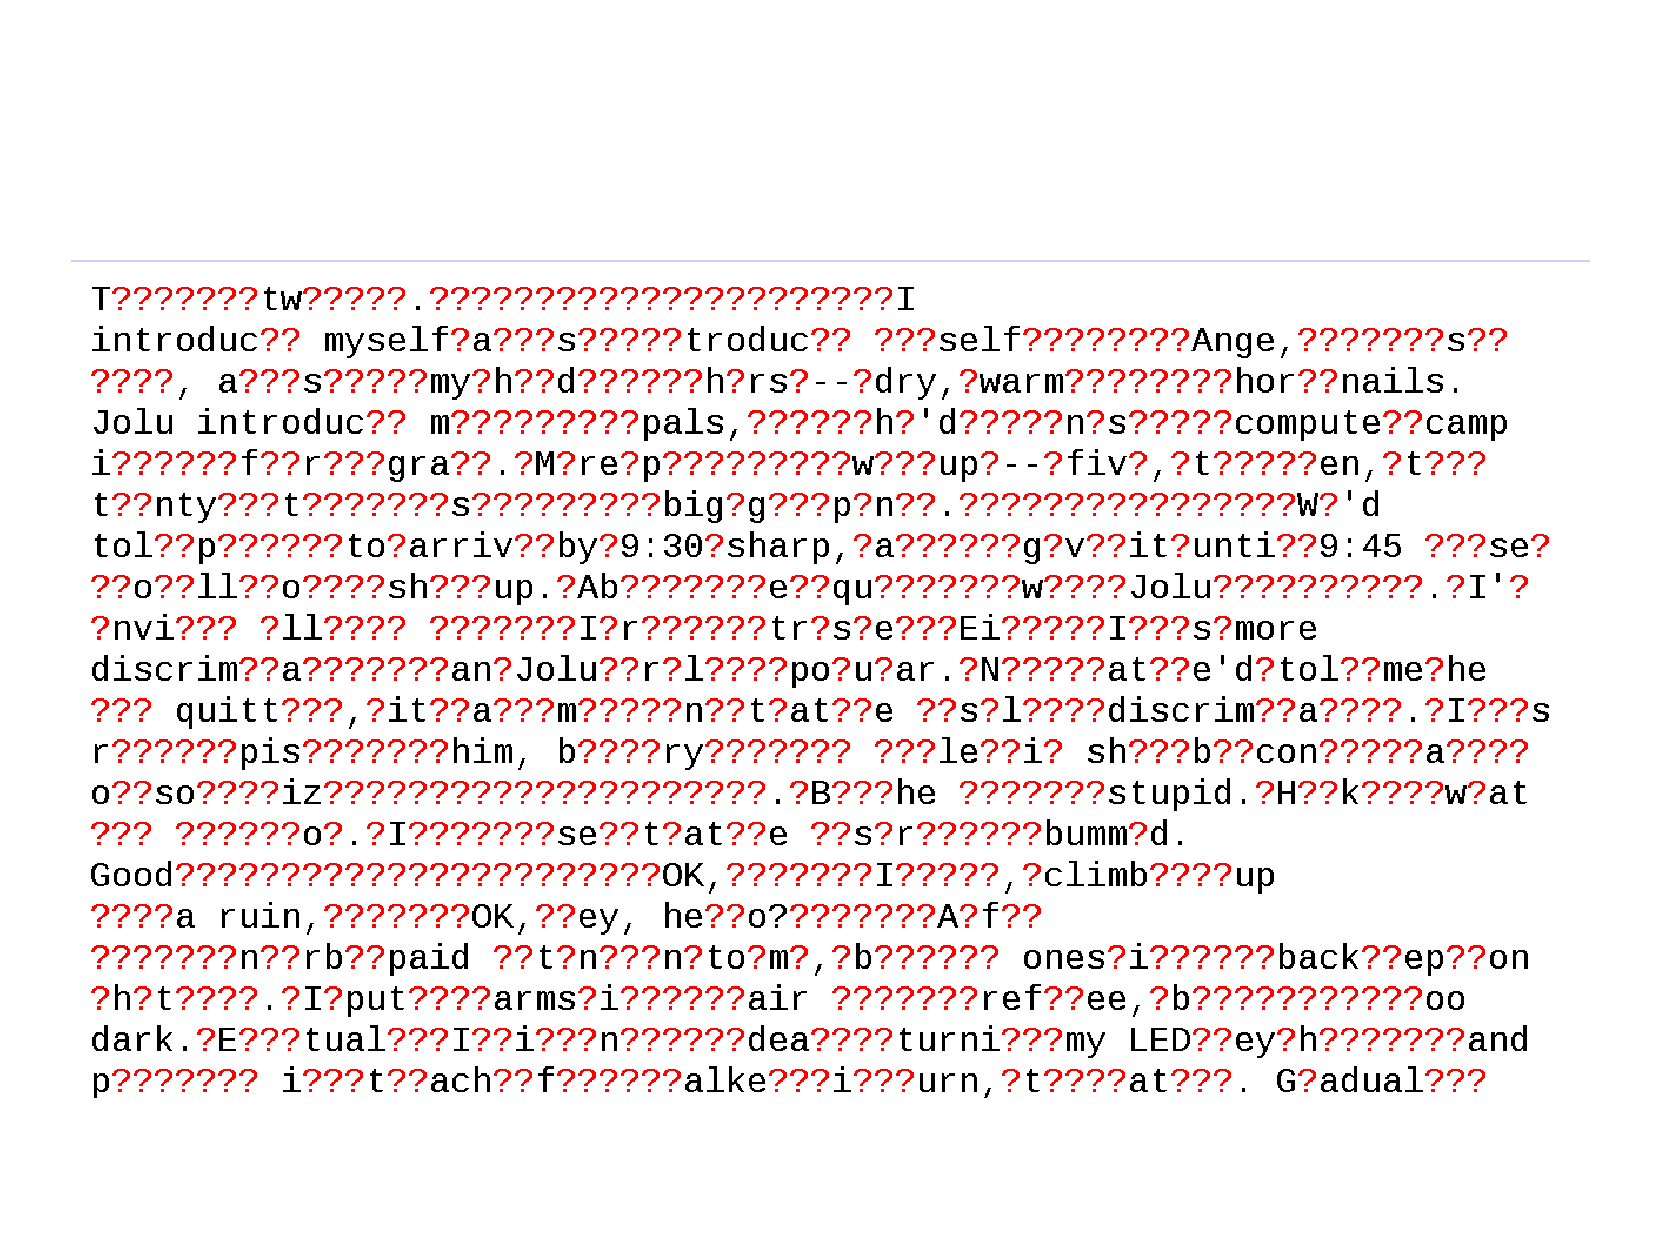
\includegraphics[width=3in]{art/brown-1} &  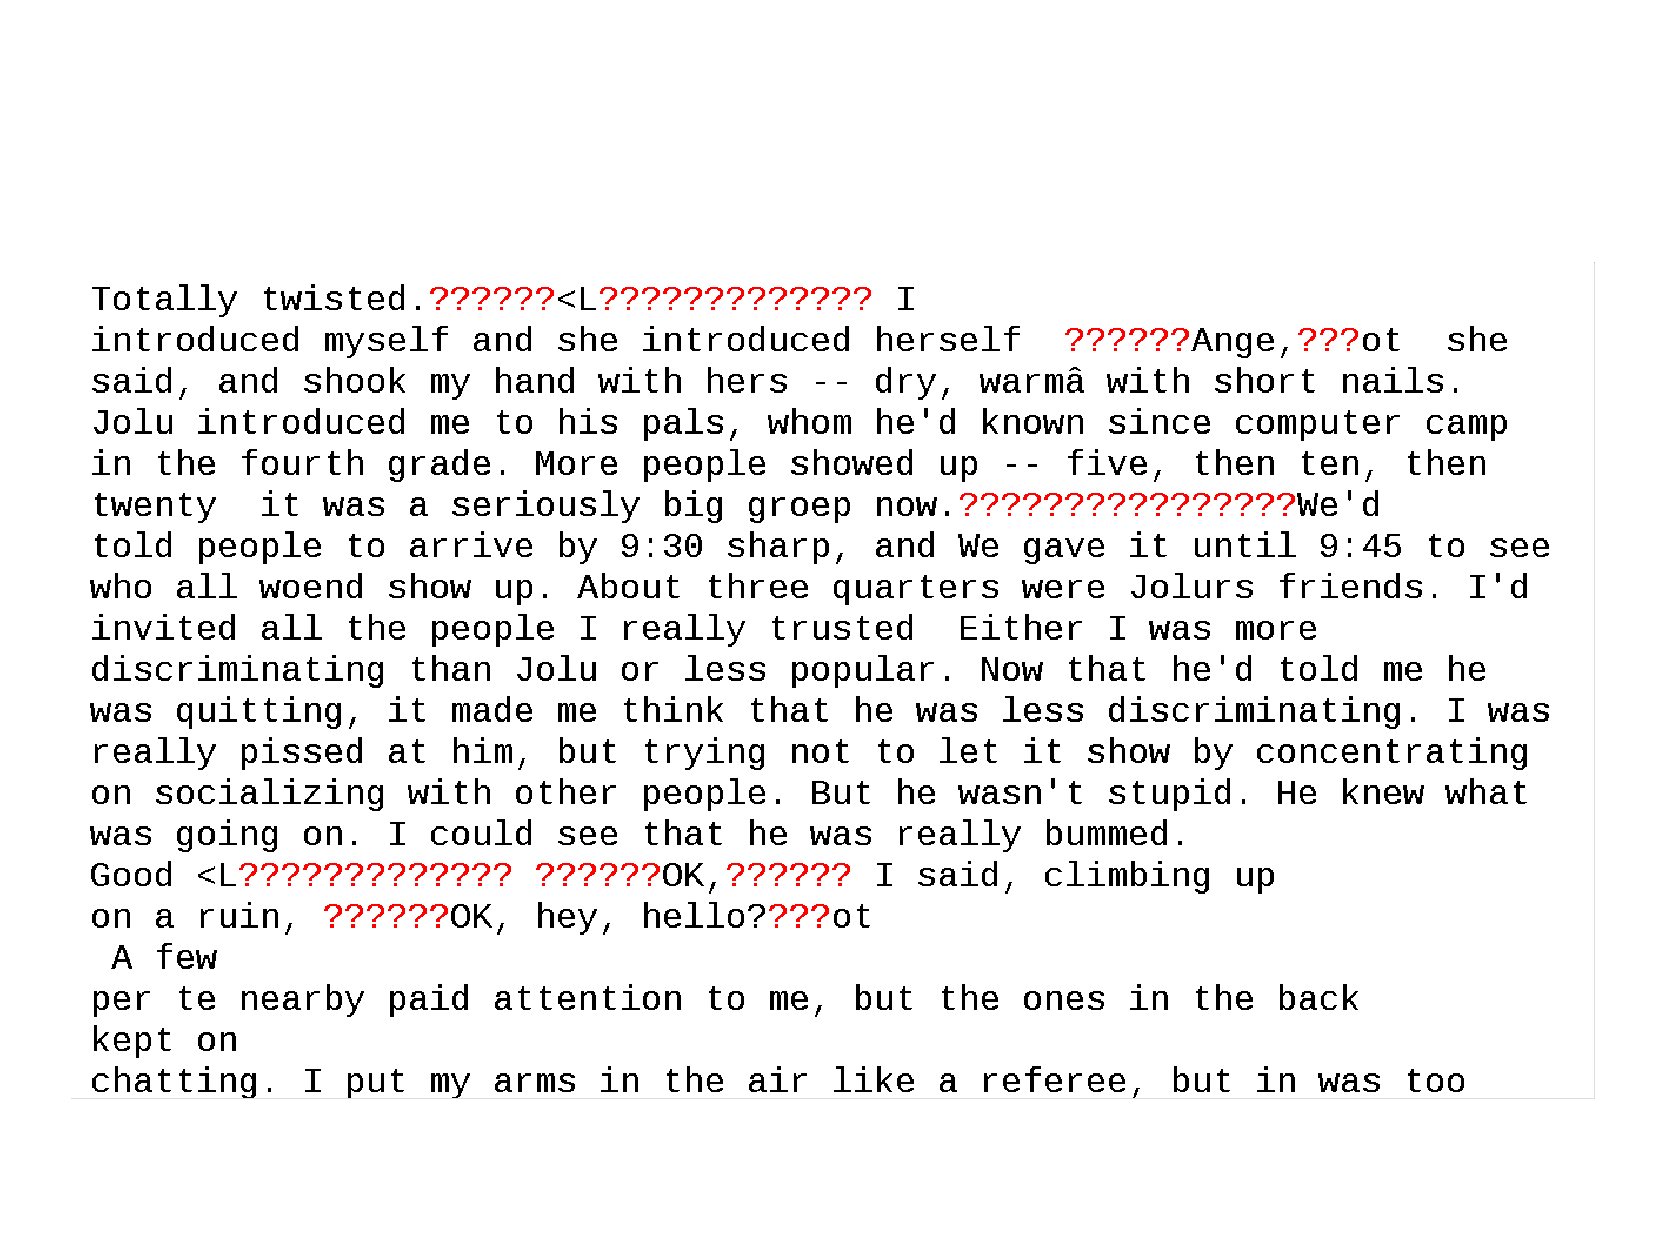
\includegraphics[width=3in]{art/brown-2} \\
\caption{Reconstructed text, without language model}\label{brown-1}
& \caption{Best possible reconstructed text, with language model}\label{brown-2}\\
\hline
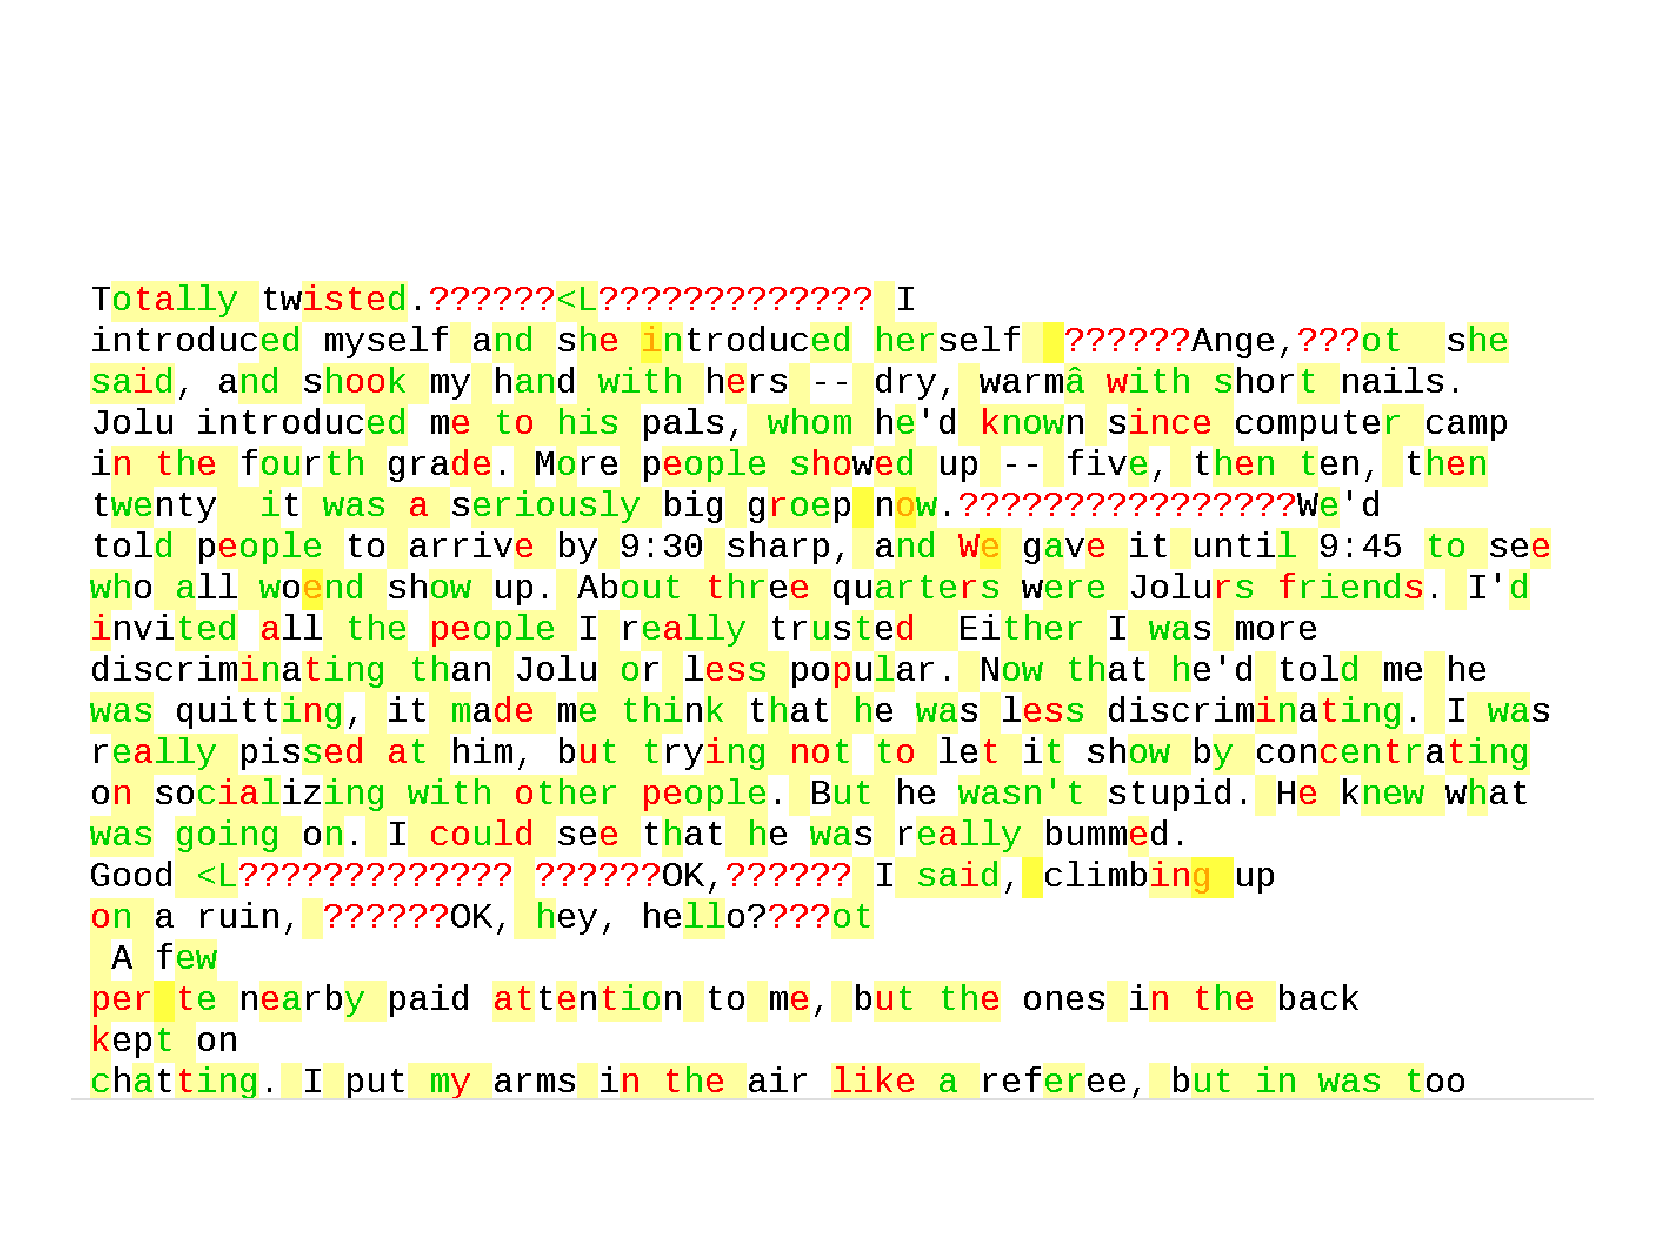
\includegraphics[width=3in]{art/brown-3} & 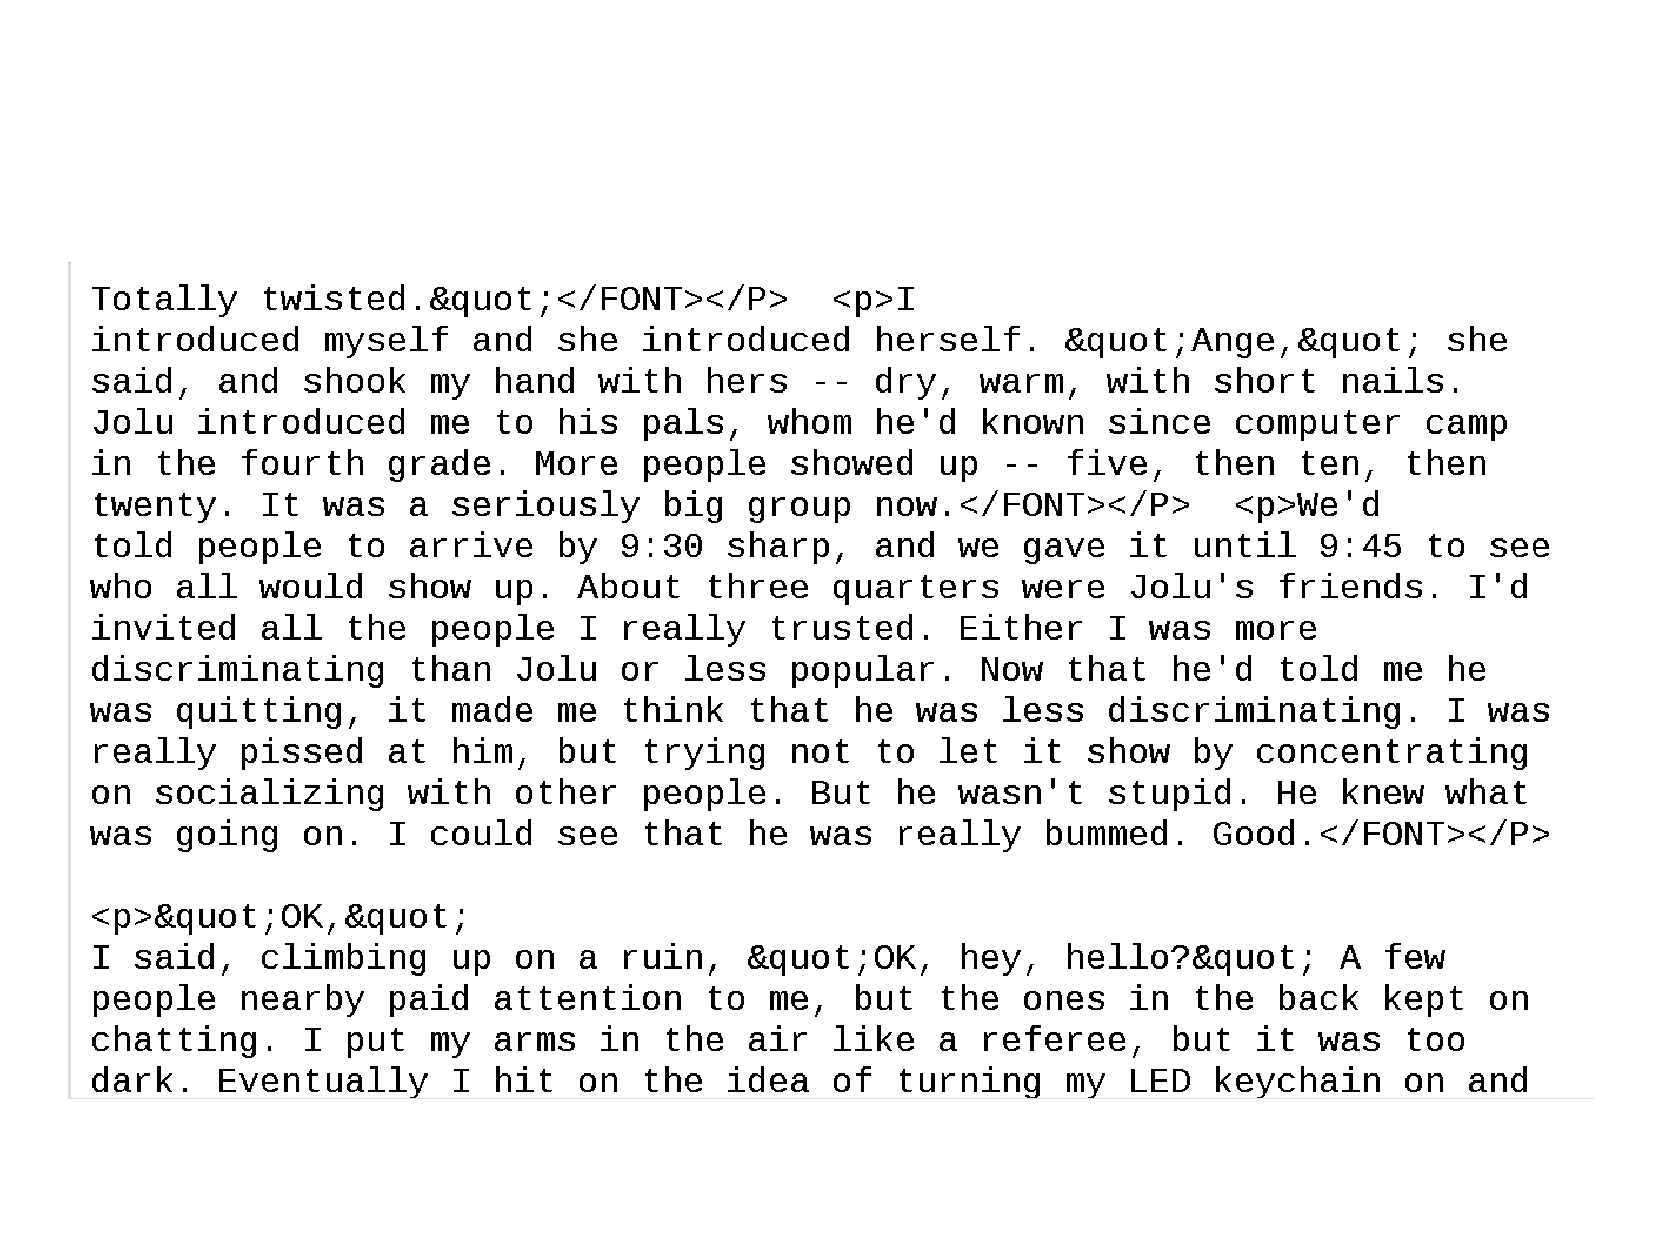
\includegraphics[width=3in]{art/brown-4}\\
\caption{Best possible reconstructed text, with language model. Green
  letters indicate high-probability matches, red letters indicate
  low-probability matches.}\label{brown-3}
&
\caption{Original text, from HTML version of Cory Doctorow novel
  ``Little Brother'', compressed using Info-Zip version 3.0, first
  1024 bytes of archive removed}\label{brown-4}
\\
\hline
\end{tabular}
\end{figure}

